\clearpage

\subsection{Comportamento in Memoria delle Liste}\label{ComportamentoInMemoriaListe}

Come già affrontato nel capitolo precedente:"\nameref{variabiliMemoria}", dove viene affrontata la questione della gestione della memoria per le variabili, anche in questo capitolo tratteremo la gestione della memoria con le liste.
\newline


Esploreremo infatti come Python gestisce le liste in memoria e come operare per ottimizzarle al meglio, e quali metodi usare a seconda dei casi d'uso.
Esploreremo concetti come \textbf{Copia profonda} e \textbf{Copia superficiale}, \textbf{Liste annidate}, il tutto relegato a come Python gestisce la memoria in questi contesti.

\vspace{0.3cm}
\subsubsection{Variabili come Riferimenti}

Come già visto nella \hyperref[variabiliMemoria]{sezione dedicata alle "variabili"} e ai riferimenti in memoria, anche per le liste il concetto di uso dei riferimenti in memoria è lo stesso, tranne per alcune eccezioni che vedremo in seguito.



\begin{lstlisting}[language=Python]
# Creazione di una lista
lista1 = [1, 2, 3]

# id() mostra l'identificatore univoco dell'oggetto in memoria
print(id(lista1))  # Ad esempio: 140424434847752
\end{lstlisting}

\subsubsection{Assegnazione e Riferimenti Multipli}

Quando assegni una lista a una seconda variabile, \textbf{non viene creata una nuova lista}, ma entrambe le variabili fanno riferimento alla stessa lista in memoria. Modificare la lista attraverso una variabile influenzerà anche l'altra.

\begin{lstlisting}[language=Python]
# Creazione di una lista
lista1 = [1, 2, 3]

# Assegnazione a una nuova variabile
lista2 = lista1  # Non crea una copia!

# Modifica attraverso lista1
lista1.append(4)

# Entrambe le liste sono state modificate
print(lista1)  # [1, 2, 3, 4]
print(lista2)  # [1, 2, 3, 4]

# Verifica che puntano allo stesso oggetto
print(id(lista1) == id(lista2))  # True
\end{lstlisting}

\begin{center}
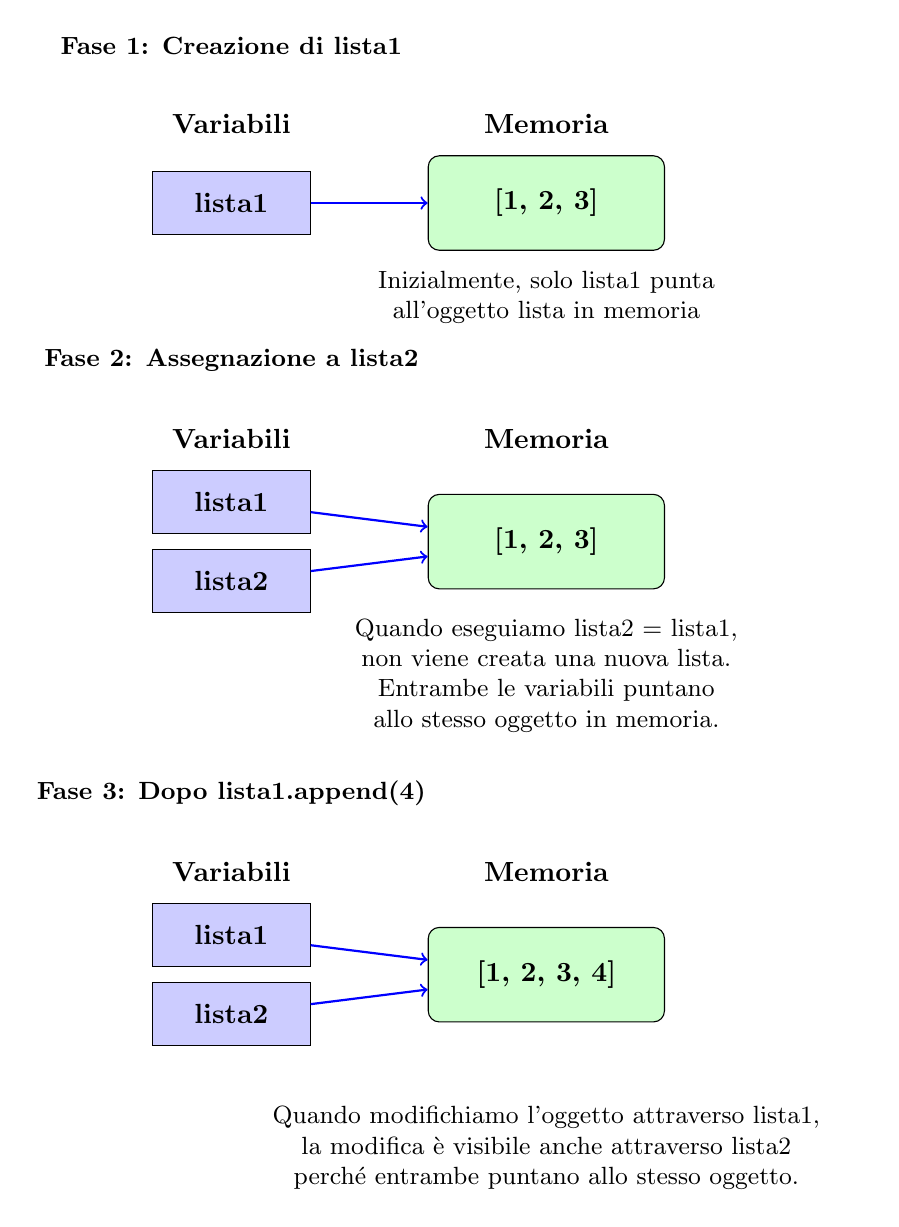
\begin{tikzpicture}
    % Definizione stili
    \tikzset{variable/.style={draw, fill=blue!20, minimum width=2cm, minimum height=0.8cm, font=\bfseries}}
    \tikzstyle{memory}=[draw, fill=green!20, minimum width=3cm, minimum height=1.2cm, rounded corners, font=\bfseries]
    \tikzstyle{reference}=[->, thick, blue]
    \tikzstyle{label}=[font=\small\bfseries]
    
    % FASE 1: Creazione di lista1
    \node[label] at (-4,2) {Fase 1: Creazione di lista1};
    
    \node[align=center, font=\bfseries] at (-4,1) {Variabili};
    \node[align=center, font=\bfseries] at (0,1) {Memoria};
    
    \node[variable = default] (var_lista1_1) at (-4,0) {lista1};
    \node[memory] (obj_lista_1) at (0,0) {[1, 2, 3]};
    \draw[reference] (var_lista1_1) -- (obj_lista_1);
    
    % FASE 2: Assegnazione a lista2
    \node[label] at (-4,-2) {Fase 2: Assegnazione a lista2};
    
    \node[align=center, font=\bfseries] at (-4,-3) {Variabili};
    \node[align=center, font=\bfseries] at (0,-3) {Memoria};
    
    \node[variable = default] (var_lista1_2) at (-4,-3.8) {lista1};
    \node[variable = default] (var_lista2_2) at (-4,-4.8) {lista2};
    \node[memory] (obj_lista_2) at (0,-4.3) {[1, 2, 3]};
    \draw[reference] (var_lista1_2) -- (obj_lista_2);
    \draw[reference] (var_lista2_2) -- (obj_lista_2);
    
    % FASE 3: Modifica con append (con più spazio)
    \node[label] at (-4,-7.5) {Fase 3: Dopo lista1.append(4)};
    
    \node[align=center, font=\bfseries] at (-4,-8.5) {Variabili};
    \node[align=center, font=\bfseries] at (0,-8.5) {Memoria};
    
    \node[variable = default] (var_lista1_3) at (-4,-9.3) {lista1};
    \node[variable = default] (var_lista2_3) at (-4,-10.3) {lista2};
    \node[memory] (obj_lista_3) at (0,-9.8) {[1, 2, 3, 4]};
    \draw[reference] (var_lista1_3) -- (obj_lista_3);
    \draw[reference] (var_lista2_3) -- (obj_lista_3);
    
    % Note esplicative
    \node[text width=8cm, align=center, font=\small] at (0,-1.2) {
        Inizialmente, solo lista1 punta all'oggetto lista in memoria
    };
    
    \node[text width=8cm, align=center, font=\small] at (0,-6) {
        Quando eseguiamo lista2 = lista1, non viene creata una nuova lista.\\ 
        Entrambe le variabili puntano allo stesso oggetto in memoria.
    };
    
    \node[text width=8cm, align=center, font=\small] at (0,-12) {
        Quando modifichiamo l'oggetto attraverso lista1,\\ 
        la modifica è visibile anche attraverso lista2\\ 
        perché entrambe puntano allo stesso oggetto.
    };
\end{tikzpicture}
\end{center}




\subsubsection{Creazione di Copie Indipendenti}
Abbiamo appena visto come, in Python, l'assegnazione di una lista ad una nuova variabile non crei una copia, ma semplicemente un nuovo riferimento allo stesso oggetto. Questo comportamento, sebbene efficiente in termini di memoria, può portare a modifiche indesiderate quando entrambe le variabili vengono utilizzate in parti diverse del codice.

Per evitare questo problema, è spesso necessario creare \textbf{copie indipendenti} delle liste, in modo che le modifiche apportate a una non influenzino l'altra. Python offre diversi metodi per creare tali copie, ciascuno con caratteristiche specifiche.

In questa sezione, esploreremo:
\begin{itemize}
    \item I metodi principali per creare copie superficiali di liste
    \item La differenza tra copia superficiale e copia profonda
    \item Quando e come utilizzare ciascun tipo di copia
    \item Gli errori comuni da evitare quando si lavora con le copie
\end{itemize}

Comprendere queste tecniche è fondamentale per scrivere codice robusto e prevedibile, specialmente in programmi di grandi dimensioni o quando si lavora con strutture dati complesse.
\newline




\paragraph{Metodi per la Creazione di Copie Indipendenti}\label{metodiCopia}
Per creare copie indipendenti di una lista, Python mette a disposizione tre metodi principali, tutti ugualmente efficaci per liste contenenti tipi di dati semplici. Vediamo questi metodi in azione e osserviamo come, dopo la modifica della lista originale, le copie mantengano i loro valori iniziali, dimostrando la loro indipendenza:

\begin{lstlisting}[language=Python]
# Creazione di una lista
originale = [1, 2, 3]
# Tre modi per creare copie
copia1 = originale.copy()       # Metodo copy() disponibile da Python 3.3
copia2 = originale[:]           # Slicing completo (funziona in tutte le versioni)
copia3 = list(originale)        # Costruttore list()
# Modifica dell'originale
originale.append(4)
# Le copie non sono influenzate
print(originale)  # [1, 2, 3, 4]
print(copia1)     # [1, 2, 3]
print(copia2)     # [1, 2, 3]
print(copia3)     # [1, 2, 3]
\end{lstlisting}

Questi tre metodi creano una \textit{copia superficiale} (shallow copy) della lista, sufficiente per la maggior parte degli usi con elementi semplici. È importante notare che, sebbene questi metodi producano lo stesso risultato in questo esempio, ciascuno ha peculiarità che potrebbero essere rilevanti in contesti più complessi, specialmente quando la lista contiene oggetti annidati.

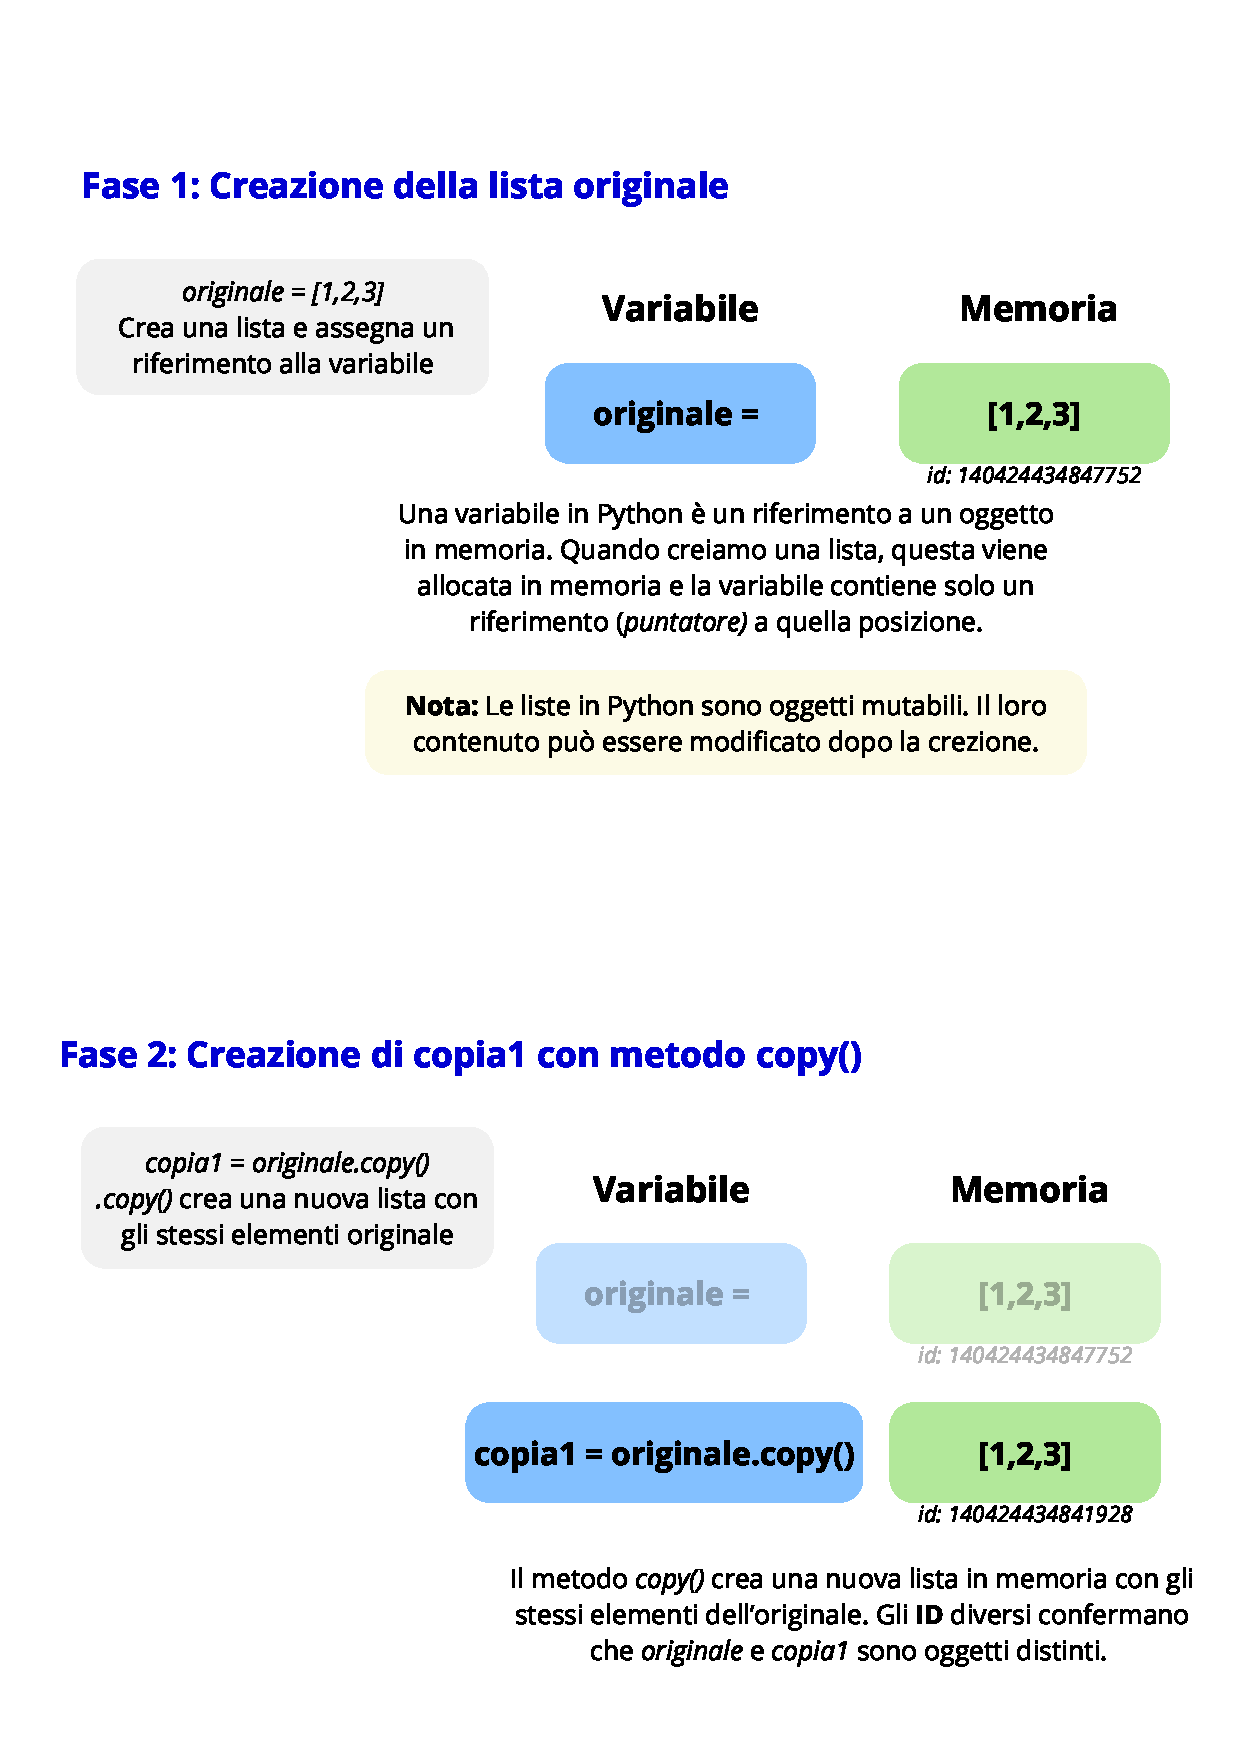
\includepdf[pages=-,scale=0.95,pagecommand={\thispagestyle{empty}},fitpaper=true]{pdf/Liste.pdf}

\paragraph{Il Problema delle Liste Annidate}\noindent

I metodi di copia visti sopra creano "copie superficiali" (shallow copies). Se la lista contiene altre liste (o oggetti mutabili), i metodi di copia standard copiano solo i riferimenti a queste liste interne, non le liste stesse. In pratica ogni modifica apportata alla lista originale, tramite \textit{shallow copies} influenzerà la sua copia.

Affrontiamo graficamente ciò che avviene con le liste annidate.

\begin{lstlisting}[language=Python]
# Lista con una lista annidata
originale = [1, 2, [3, 4]]

# Creazione di una copia superficiale
copia = originale.copy()

# Modifica della lista interna nell'originale
originale[2].append(5)

# La modifica si riflette anche nella copia!
print(originale)  # [1, 2, [3, 4, 5]]
print(copia)      # [1, 2, [3, 4, 5]]
\end{lstlisting}

\begin{center}
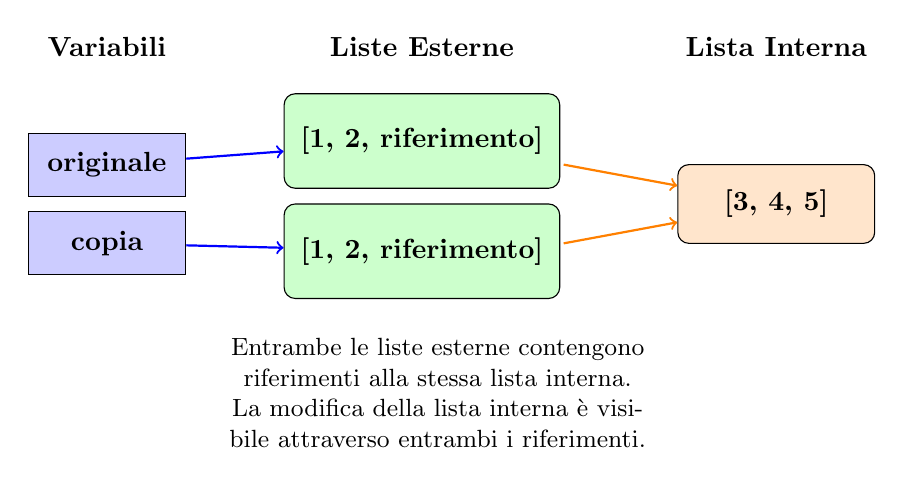
\begin{tikzpicture}
    % Definizione stili
    \tikzstyle{variable}=[draw, fill=blue!20, minimum width=2cm, minimum height=0.8cm, font=\bfseries]
    \tikzstyle{memory}=[draw, fill=green!20, minimum width=3.5cm, minimum height=1.2cm, rounded corners, font=\bfseries]
    \tikzstyle{innermemory}=[draw, fill=orange!20, minimum width=2.5cm, minimum height=1cm, rounded corners, font=\bfseries]
    \tikzstyle{reference}=[->, thick, blue]
    \tikzstyle{innerref}=[->, thick, orange]
    
    % Etichette per le sezioni
    \node[align=center, font=\bfseries] at (0,2.5) {Variabili};
    \node[align=center, font=\bfseries] at (4,2.5) {Liste Esterne};
    \node[align=center, font=\bfseries] at (8.5,2.5) {Lista Interna};
    
    % Variabili
    \node[variable = default] (var_orig) at (0,1) {originale};
    \node[variable = default] (var_copia) at (0,0) {copia};
    
    % Oggetti lista esterna in memoria
    \node[memory] (obj_orig) at (4,1.3) {[1, 2, riferimento]};
    \node[memory] (obj_copia) at (4,-0.1) {[1, 2, riferimento]};
    
    % Oggetto lista interna in memoria
    \node[innermemory] (obj_inner) at (8.5,0.5) {[3, 4, 5]};
    
    % Frecce di riferimento esterne
    \draw[reference] (var_orig) -- (obj_orig);
    \draw[reference] (var_copia) -- (obj_copia);
    
    % Frecce di riferimento interne
    \draw[innerref] (5.8,1) -- (obj_inner);
    \draw[innerref] (5.8,0) -- (obj_inner);
    
    % Spiegazione
    \node[text width=10cm, font=\small, align=center] at (4.2,-1.9) {
        Entrambe le liste esterne contengono riferimenti alla stessa lista interna.\\
        La modifica della lista interna è visibile attraverso entrambi i riferimenti.
    };
\end{tikzpicture}
\end{center}

\paragraph{Il Problema della Copia profonda in Dettaglio}

Come abbiamo accennato sopra \textit{"\nameref{metodiCopia}"}, sono metodi che creano una copia superficiale. Questo approccio presenta limitazioni significative quando si lavora con strutture di dati annidate:

\subparagraph{Comprensione del Problema}

Le copie superficiali duplicano solo la struttura esterna, mantendendo i riferimenti agli stessi oggetti interni.


% Fase 1: Confronto tra copia superficiale e copia profonda prima delle modifiche
\begin{figure}[htbp]
    \centering
    \begin{tikzpicture}[node distance=1.5cm]
        % Titolo
        \node[section title] at (0,2) {Fase 1: Confronto tra copia superficiale e copia profonda};
        
        % Etichette colonne
        \node[label] at (-4,1) {Variabile};
        \node[label] at (0,1) {Lista Esterna};
        \node[label] at (4,1) {Lista Interna};
        
        % Originale
        \node[variable={default}] (var_orig) at (-4,0) {originale};
        \node[memory] (mem_orig) at (0,0) {[1, 2, riferimento]};
        \node[memory] (mem_inner) at (4,0) {[3, 4]};
        \draw[reference] (var_orig) -- (mem_orig);
        \draw[reference] (mem_orig) -- (mem_inner);
        \node[id label] at (0,-0.8) {id: 140424434847752};
        \node[id label] at (4,-0.8) {id: 140424434830280};
        
        % Copia superficiale
        \node[variable={default}] (var_shallow) at (-4,-2) {copia\_superficiale};
        \node[memory] (mem_shallow) at (0,-2) {[1, 2, riferimento]};
        \draw[reference] (var_shallow) -- (mem_shallow);
        \draw[reference] (mem_shallow) to[out=0, in=190] (mem_inner);
        \node[id label] at (0,-2.8) {id: 140424434841928};
        
        % Copia profonda
        \node[variable={default}] (var_deep) at (-4,-4) {copia\_profonda};
        \node[memory] (mem_deep) at (0,-4) {[1, 2, riferimento]};
        \node[memory] (mem_inner_deep) at (4,-4) {[3, 4]};
        \draw[reference] (var_deep) -- (mem_deep);
        \draw[reference] (mem_deep) -- (mem_inner_deep);
        \node[id label] at (0,-4.8) {id: 140424434836104};
        \node[id label] at (4,-4.8) {id: 140424434825456};
        
        % Spiegazione
        \node[explanation] at (0,-6.5) {Confronto tra copie: la copia superficiale crea un nuovo oggetto 
        lista esterna ma mantiene il riferimento alla stessa lista interna dell'originale. 
        La copia profonda duplica sia la lista esterna che quella interna, creando oggetti completamente indipendenti.};
    \end{tikzpicture}
    \caption{Confronto tra copia superficiale e copia profonda prima della modifica}
    \label{fig:deep-copy-before}
\end{figure}

% Fase 2: Comportamento dopo la modifica
\begin{figure}[htbp]
    \centering
    \begin{tikzpicture}[node distance=1.5cm]
        % Titolo
        \node[section title] at (0,2) {Fase 2: Effetto delle modifiche sulla lista interna};
        
        % Etichette colonne
        \node[label] at (-4,1) {Variabile};
        \node[label] at (0,1) {Lista Esterna};
        \node[label] at (4,1) {Lista Interna};
        
        % Originale
        \node[variable={default}] (var_orig) at (-4,0) {originale};
        \node[memory] (mem_orig) at (0,0) {[1, 2, riferimento]};
        \node[memory] (mem_inner) at (4,0) {[3, 4, 5]};
        \draw[reference] (var_orig) -- (mem_orig);
        \draw[reference] (mem_orig) -- (mem_inner);
        \node[id label] at (0,-0.8) {id: 140424434847752};
        \node[id label] at (4,-0.8) {id: 140424434830280};
        
        % Copia superficiale
        \node[variable={default}] (var_shallow) at (-4,-2) {copia\_superficiale};
        \node[memory] (mem_shallow) at (0,-2) {[1, 2, riferimento]};
        \draw[reference] (var_shallow) -- (mem_shallow);
        \draw[reference] (mem_shallow) to[out=0, in=190] (mem_inner);
        \node[id label] at (0,-2.8) {id: 140424434841928};
        
        % Copia profonda
        \node[variable={default}] (var_deep) at (-4,-4) {copia\_profonda};
        \node[memory] (mem_deep) at (0,-4) {[1, 2, riferimento]};
        \node[memory] (mem_inner_deep) at (4,-4)  {[3, 4]};
        \draw[reference] (var_deep) -- (mem_deep);
        \draw[reference] (mem_deep) -- (mem_inner_deep);
        \node[id label] at (0,-4.8) {id: 140424434836104};
        \node[id label] at (4,-4.8) {id: 140424434825456};
        
        % Spiegazione
        \node[explanation] at (0,-6.5) {Dopo aver modificato la lista interna dell'originale con \texttt{originale[2].append(5)}, 
        la modifica si riflette anche nella copia superficiale perché entrambi condividono lo stesso oggetto interno. 
        La copia profonda rimane invariata perché contiene una duplicazione indipendente della lista interna.};
        
        % Evidenziazione della modifica
        \draw[red, thick, dashed] (4,0.04) circle (0.62);
        \node[red, font=\small\bfseries] at (3.2,-1.4) {Modificato};

        % Evidenziazione dell'effetto sulla copia superficiale  
        \draw[red, ->, thick, dashed] (6.5,-1) -- (5.1,-0.1);
        \node[red, text width=2.5cm, align=center, font=\small\bfseries] at (7.5,-1) {La modifica si riflette anche qui};
        
        % Evidenziazione dell'indipendenza della copia profonda
        \draw[green!60!black, ->, thick, dashed] (6.5,-4) -- (5.1,-4);
        \node[green!60!black, text width=2.5cm, align=center, font=\small\bfseries] at (7.5,-4) {Rimane invariata};
    \end{tikzpicture}
    \caption{Effetto delle modifiche: differenza tra copia superficiale e profonda}
    \label{fig:deep-copy-after}
\end{figure}

\newpage
\paragraph{Copie Profonde}

Per creare una "copia profonda" (deep copy) che copia anche gli oggetti annidati, si può utilizzare il modulo \texttt{copy}:

\begin{lstlisting}[language=Python]
import copy

# Lista con una lista annidata
originale = [1, 2, [3, 4]]

# Creazione di una copia profonda
copia_profonda = copy.deepcopy(originale)

# Modifica della lista interna nell'originale
originale[2].append(5)

# La copia profonda non è influenzata
print(originale)      # [1, 2, [3, 4, 5]]
print(copia_profonda) # [1, 2, [3, 4]]
\end{lstlisting}

\begin{center}
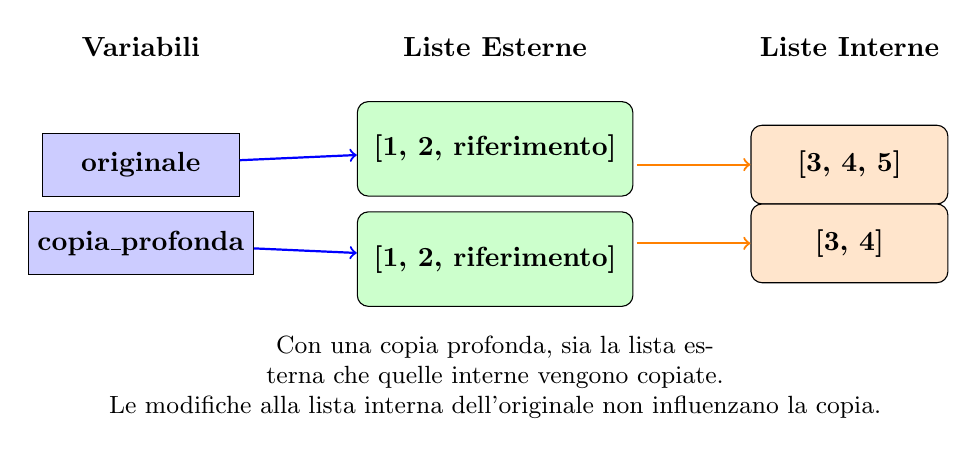
\begin{tikzpicture}
    % Definizione stili
    \tikzstyle{variable}=[draw, fill=blue!20, minimum width=2.5cm, minimum height=0.8cm, font=\bfseries]
    \tikzstyle{memory}=[draw, fill=green!20, minimum width=3.5cm, minimum height=1.2cm, rounded corners, font=\bfseries]
    \tikzstyle{innermemory}=[draw, fill=orange!20, minimum width=2.5cm, minimum height=1cm, rounded corners, font=\bfseries]
    \tikzstyle{reference}=[->, thick, blue]
    \tikzstyle{innerref}=[->, thick, orange]
    
    % Etichette per le sezioni
    \node[align=center, font=\bfseries] at (-0.5,2.5) {Variabili};
    \node[align=center, font=\bfseries] at (4,2.5) {Liste Esterne};
    \node[align=center, font=\bfseries] at (8.5,2.5) {Liste Interne};
    
    % Variabili
    \node[variable = default = default] (var_orig) at (-0.5,1) {originale};
    \node[variable = default] (var_copia) at (-0.5,0) {copia\_profonda};
    
    % Oggetti lista esterna in memoria
    \node[memory] (obj_orig) at (4,1.2) {[1, 2, riferimento]};
    \node[memory] (obj_copia) at (4,-0.2) {[1, 2, riferimento]};
    
    % Oggetti lista interna in memoria
    \node[innermemory] (obj_inner_orig) at (8.5,1) {[3, 4, 5]};
    \node[innermemory] (obj_inner_copia) at (8.5,0) {[3, 4]};
    
    % Frecce di riferimento esterne
    \draw[reference] (var_orig) -- (obj_orig);
    \draw[reference] (var_copia) -- (obj_copia);
    
    % Frecce di riferimento interne
    \draw[innerref] (5.8,1) -- (obj_inner_orig);
    \draw[innerref] (5.8,0) -- (obj_inner_copia);
    
    % Spiegazione
    \node[text width=10cm, font=\small, align=center] at (4,-1.7) {
        Con una copia profonda, sia la lista esterna che quelle interne vengono copiate.\\
        Le modifiche alla lista interna dell'originale non influenzano la copia.
    };
\end{tikzpicture}
\end{center}


\subsubsection{Confronto tra Liste: `==` vs `is`}\label{ConfrontoOperatoriListe}

Python fornisce due modi per confrontare le liste:
\begin{itemize}
    \item L'operatore \texttt{==} confronta il contenuto delle liste (uguaglianza di valore)
    \item L'operatore \texttt{is} confronta gli identificatori degli oggetti (uguaglianza di identità)
\end{itemize}

\begin{lstlisting}[language=Python]
a = [1, 2, 3]
b = [1, 2, 3]  # Una nuova lista con gli stessi valori
c = a          # Riferimento alla stessa lista

print(a == b)  # True - stesso contenuto
print(a is b)  # False - oggetti diversi in memoria
print(a is c)  # True - stesso oggetto in memoria
\end{lstlisting}

\subsubsection{Rappresentazione Visiva della Memoria}



\begin{lstlisting}[language=Python]
a = [1, 2, 3]
b = [1, 2, 3]  # Una nuova lista con gli stessi valori
c = a          # Riferimento alla stessa lista

print(a == b)  # True - stesso contenuto
print(a is b)  # False - oggetti diversi in memoria
print(a is c)  # True - stesso oggetto in memoria

# Visualizzazione degli id per conferma
print(id(a))  # Ad esempio: 140424434847752
print(id(b))  # Diverso da a
print(id(c))  # Stesso di a
\end{lstlisting}

\begin{center}
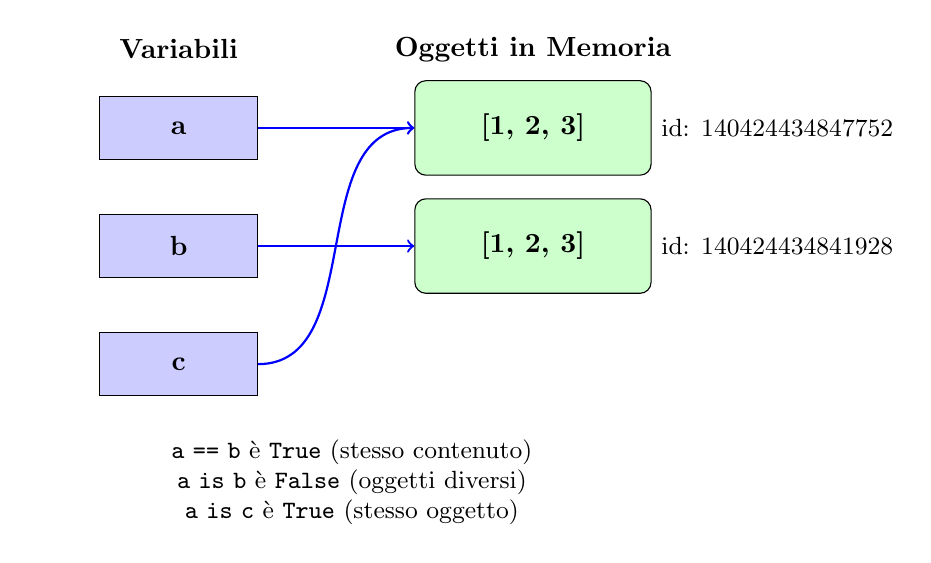
\begin{tikzpicture}
    % Definizione stili
    \tikzstyle{variable}=[draw, fill=blue!20, minimum width=2cm, minimum height=0.8cm, font=\bfseries]
    \tikzstyle{memory}=[draw, fill=green!20, minimum width=3cm, minimum height=1.2cm, rounded corners, font=\bfseries]
    \tikzstyle{reference}=[->, thick, blue]
    
    % Etichette per le sezioni
    \node[align=center, font=\bfseries] at (0,3) {Variabili};
    \node[align=center, font=\bfseries] at (4.5,3) {Oggetti in Memoria};
    
    % Variabili
    \node[variable = default] (var_a) at (0,2) {a};
    \node[variable = default] (var_b) at (0,0.5) {b};
    \node[variable = default] (var_c) at (0,-1) {c};
    
    % Oggetti in memoria
    \node[memory] (obj_a) at (4.5,2) {[1, 2, 3]};
    \node[memory] (obj_b) at (4.5,0.5) {[1, 2, 3]};
    
    % IDs
    \node[right, font=\small] at (obj_a.east) {id: 140424434847752};
    \node[right, font=\small] at (obj_b.east) {id: 140424434841928};
    
    % Frecce di riferimento
    \draw[reference] (var_a) -- (obj_a);
    \draw[reference] (var_b) -- (obj_b);
    \draw[reference] (var_c) to [out=0, in=180] (obj_a);
    
    % Spiegazione
    \node[text width=8cm, font=\small, align=center] at (2.2,-2.5) {
        \texttt{a == b} è \texttt{True} (stesso contenuto)\\
        \texttt{a is b} è \texttt{False} (oggetti diversi)\\
        \texttt{a is c} è \texttt{True} (stesso oggetto)
    };
\end{tikzpicture}
\end{center}

\paragraph{Errore Comune: Liste Annidate Moltiplicate}

Un errore comune quando si lavora con liste annidate è la creazione di matrici usando la moltiplicazione di liste:

\begin{lstlisting}[language=Python]
# Tentativo ERRATO di creare una matrice 3x3 di zeri
matrice_errata = [[0] * 3] * 3
print(matrice_errata)  # [[0, 0, 0], [0, 0, 0], [0, 0, 0]]

# Modifica di un solo elemento
matrice_errata[0][0] = 1
print(matrice_errata)  # [[1, 0, 0], [1, 0, 0], [1, 0, 0]]  Oops!
\end{lstlisting}

Cosa è successo? L'espressione `[[0] * 3] * 3` crea una lista contenente tre riferimenti alla stessa lista interna. Quando modifichi un elemento in una "riga", la modifica appare in tutte le righe perché puntano allo stesso oggetto.

\begin{center}
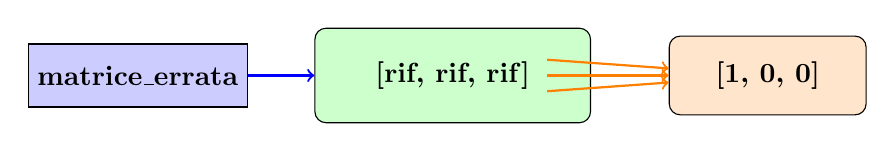
\begin{tikzpicture}
    % Definizione stili
    \tikzstyle{variable}=[draw, fill=blue!20, minimum width=2cm, minimum height=0.8cm, font=\bfseries]
    \tikzstyle{memory}=[draw, fill=green!20, minimum width=3.5cm, minimum height=1.2cm, rounded corners, font=\bfseries]
    \tikzstyle{innermemory}=[draw, fill=orange!20, minimum width=2.5cm, minimum height=1cm, rounded corners, font=\bfseries]
    \tikzstyle{reference}=[->, thick, blue]
    \tikzstyle{innerref}=[->, thick, orange]
    
    % Variabile
    \node[variable = default] (var_matrice) at (0,0) {matrice\_errata};
    
    % Oggetto lista esterna in memoria
    \node[memory] (obj_matrice) at (4,0) {[rif, rif, rif]};
    
    % Oggetto lista interna in memoria (una sola lista per tutte e 3 le righe!)
    \node[innermemory] (obj_inner) at (8,0) {[1, 0, 0]};
    
    % Frecce di riferimento esterne
    \draw[reference] (var_matrice) -- (obj_matrice);
    
    % Frecce di riferimento interne - tutte puntano alla stessa lista interna!
    \draw[innerref] (5.2,0.2) -- (obj_inner);
    \draw[innerref] (5.2,0) -- (obj_inner);
    \draw[innerref] (5.2,-0.2) -- (obj_inner);
\end{tikzpicture}
\end{center}

\paragraph{Soluzione Corretta}

Il modo corretto per creare liste annidate indipendenti è utilizzare una comprensione di lista:

\begin{lstlisting}[language=Python]
# Modo CORRETTO:
matrice_corretta = [[0 for _ in range(3)] for _ in range(3)]
matrice_corretta[0][0] = 1
print(matrice_corretta)  # [[1, 0, 0], [0, 0, 0], [0, 0, 0]]
\end{lstlisting}

\begin{center}
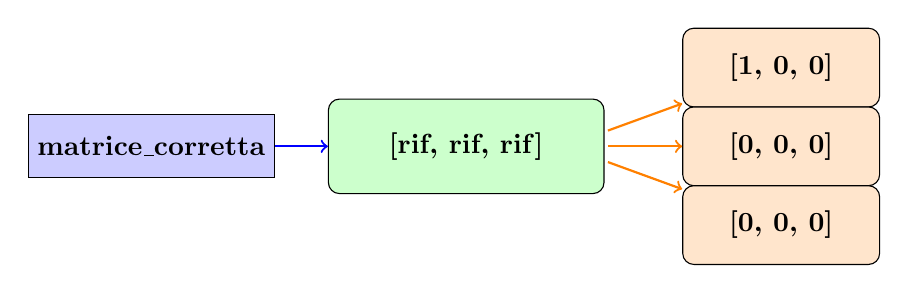
\begin{tikzpicture}
    % Definizione stili
    \tikzstyle{variable}=[draw, fill=blue!20, minimum width=2.5cm, minimum height=0.8cm, font=\bfseries]
    \tikzstyle{memory}=[draw, fill=green!20, minimum width=3.5cm, minimum height=1.2cm, rounded corners, font=\bfseries]
    \tikzstyle{innermemory}=[draw, fill=orange!20, minimum width=2.5cm, minimum height=1cm, rounded corners, font=\bfseries]
    \tikzstyle{reference}=[->, thick, blue]
    \tikzstyle{innerref}=[->, thick, orange]
    
    % Variabile
    \node[variable = default] (var_matrice) at (0,0) {matrice\_corretta};
    
    % Oggetto lista esterna in memoria
    \node[memory] (obj_matrice) at (4,0) {[rif, rif, rif]};
    
    % Oggetti lista interna in memoria (tre liste diverse!)
    \node[innermemory] (row1) at (8,1) {[1, 0, 0]};
    \node[innermemory] (row2) at (8,0) {[0, 0, 0]};
    \node[innermemory] (row3) at (8,-1) {[0, 0, 0]};
    
    % Frecce di riferimento esterne
    \draw[reference] (var_matrice) -- (obj_matrice);
    
    % Frecce di riferimento interne - ciascuna punta a una lista diversa
    \draw[innerref] (5.8,0.2) -- (row1);
    \draw[innerref] (5.8,0) -- (row2);
    \draw[innerref] (5.8,-0.2) -- (row3);
\end{tikzpicture}
\end{center}

In questo caso, ogni riga è un oggetto lista separato e indipendente. Modificando un elemento in una riga, le altre righe non sono influenzate.

\paragraph{Implicazioni Pratiche}

Comprendere come funzionano i riferimenti in Python ha importanti implicazioni pratiche:

\begin{itemize}
    \item \textbf{Modifiche indesiderate}: Modificare una lista attraverso un riferimento influenza tutti i riferimenti alla stessa lista
    \item \textbf{Copie superficiali non sufficienti}: Quando la lista contiene oggetti mutabili, una copia superficiale potrebbe non essere sufficiente
    \item \textbf{Confronto con \texttt{is}}: Utilizzare \texttt{is} quando si intende confrontare il contenuto può portare a risultati inaspettati
\end{itemize}
\begin{center}

\end{center}

\subsubsection{Implicazioni Pratiche}

Comprendere come funzionano i riferimenti in Python ha importanti implicazioni pratiche:

\begin{tcolorbox}[colback=red!5!white,colframe=red!75!black,title=Errori comuni con i riferimenti alle liste]
\begin{itemize}
    \item \textbf{Modifiche indesiderate}: Modificare una lista attraverso un riferimento influenza tutti i riferimenti alla stessa lista
    \item \textbf{Copie superficiali non sufficienti}: Quando la lista contiene oggetti mutabili, una copia superficiale potrebbe non essere sufficiente
    \item \textbf{Confronto con \texttt{is}}: Utilizzare \texttt{is} quando si intende confrontare il contenuto può portare a risultati inaspettati
\end{itemize}
\end{tcolorbox}